% Drawing 154/02-3 -- folder 154, batch 02, archive page 22 (PDF page 23).
% Transcription: figure : deux faisceaux de pseudo-droites orange sur une droite verte, un trait épais noir marquant sur celle-ci l'arc intercepté par chacun
% Kind: two pencils on a line, intercepted arcs. Method 2 (schematic redraw from the facsimile). Status: ok.
% Notes: Two pencils of orange pseudolines on a green line (four lines on the left, three on the right); a thick black stroke on the green line marks the arc intercepted by each.
% Coordinates: 1 unit = 1 mm = 1/100 of the crop width (bbox in page fractions: [0.152, 0.114, 0.393, 0.201]).
% Redrawn by Claude (claude-opus-5-5), issue #73, 2026-11-07; not checked by a human; not compiled (no TeX in the session).
% Revised by Claude (claude-opus-5-5) 2026-11-09 (issue #128) after Michel's check: vertices snapped to exact intersections (drawn points on their lines, meeting ends on the stroke they meet, near-concurrent lines through one computed point, curve ends on their rim); labels at \small as in folder 80 batch 3. Status: ok.
% Rights: reproduces part of the work -- behind RENDER_TRANSCRIPTS, never published by itself.
\documentclass[tikz,border=3pt]{standalone}
\usepackage{amsmath,amssymb}
\usetikzlibrary{patterns,arrows.meta}
\tikzset{Or/.style={orange!90!black}, Ye/.style={yellow!80!orange}, Lg/.style={green!60!black!70}, Dg/.style={green!45!black}, Br/.style={brown!80!black}, Rd/.style={red!85!black}, Bl/.style={blue!70!black}, Gy/.style={black!40}, pencil/.style={black!45}, struck/.style={black!35}, mark/.style={circle,draw,inner sep=1.3pt}, pt/.style={circle,fill,inner sep=0.9pt}, opt/.style={circle,draw,fill=white,inner sep=1.1pt}}
\colorlet{Or}{orange!90!black}\colorlet{Ye}{yellow!80!orange}\colorlet{Lg}{green!60!black!70}\colorlet{Dg}{green!45!black}\colorlet{Br}{brown!80!black}\colorlet{Rd}{red!85!black}\colorlet{Bl}{blue!70!black}\colorlet{Gy}{black!40}
\begin{document}
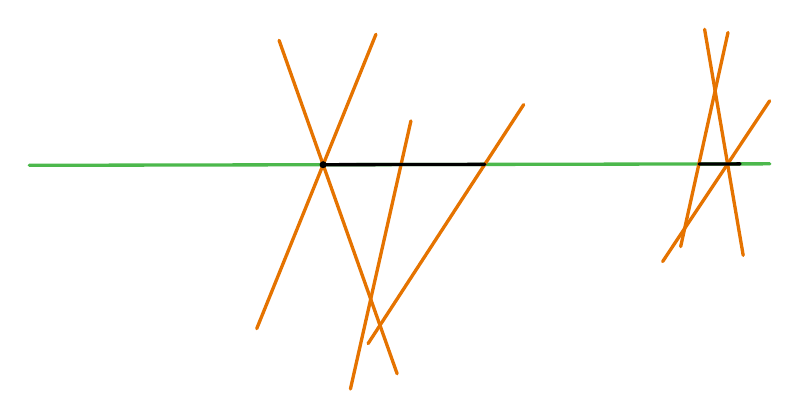
\begin{tikzpicture}[x=1mm,y=1mm,line cap=round,line join=round,font=\scriptsize]
\draw[Lg,very thick] (2.55,-20.27) -- (96.59,-20.08);
\draw[Or,very thick] (34.27,-4.4) -- (49.26,-46.74);
\draw[Or,very thick] (46.57,-3.63) -- (31.43,-41.01);
\draw[Or,very thick] (51.01,-14.63) -- (43.33,-48.68);
\draw[Or,very thick] (65.33,-12.56) -- (45.57,-42.91);
\draw[Or,very thick] (88.31,-3) -- (93.21,-31.7);
\draw[Or,very thick] (91.28,-3.4) -- (85.27,-30.59);
\draw[Or,very thick] (96.57,-12.08) -- (82.98,-32.49);
\draw[very thick] (39.86,-20.19) -- (60.39,-20.15);
\node[pt] at (39.86,-20.19) {};
\draw[very thick] (87.59,-20.1) -- (92.81,-20.09);
\end{tikzpicture}
\end{document}
